\chapter{Implementierung}

\anno{max. 5 Seiten (7)} %Ref hat 12

% Was lesen wir in diesem Kapitel?
% Warum muss ich das als Gutachter lesen
% Wie verknüpft sich der Inhalt mit dem vorhergehenden Kapitel?
% Welche Implmentierungsentscheidungen? Welche Alternativen? Vor- und Nachteile des eigenen Ansatzes?

% Highlight 1 der Implementierung
Wie bereits in Abschnitt \ref{sec:Probleme} angemerkt sind offene Implementationen von Web Application Firewalls eher die Ausnahme und selbst Umsetzungen der in Abschnitt \ref{sec:relatedwork} erwähnten Produkte sind praktisch nicht auffindbar. In diesem Kapitel gibt es einen kurzen Überblick wie die Vorschläge aus dem vorhergehenden Kapitel dennoch praktisch umgesetzt werden können.

Eine komplette Umsetzung ohne vorherige Basis wäre zeitlich (von einer einzelnen Person) nicht umsetzbar gewesen, daher sollte ein vorhandenes Open Source Produkt entsprechend erweitert werden. Bei der Auswahl wurden zuerst die zwei (leichtgewichtigen) Lösungen \emph{OWASP ESAPIFilter}\footnote{\url{https://owasp.org/www-project-enterprise-security-api/} abgerufen am 05.07.2023} und {SpringSecurity HttpFirewall}\footnote{\url{https://docs.spring.io/spring-security/reference/servlet/exploits/firewall.html} abgerufen am 05.07.2023} betrachtet. Beide Produkte verstehen sich als Ausgangsbasis für die Entwicklung sicherheitsrelevanter HTTP-(Servlet)-Filter auf Anwendungsebene, sämtliche Funktionalität muss jedoch vom Nutzer erst implementiert werden. Bei der Nutzung wäre ein erhöhter Arbeitsaufwand absehbar. Diogo Sampaio und Jorge Bernardino verglichen 2017 verfügbare WAFs die ebenfalls als Erweiterungskandidaten in Frage kamen (siehe Tabelle \ref{tab:my_vergos}).

% Tabelle ggf. in Anhang verschieben

\begin{table}[h]
  \centering
  \begin{tabular}{lccc} 
    \toprule
    & \textbf{ModSecurity} & \textbf{WebCastellum} & \textbf{IronBee} \\ [0.5ex] 
    \midrule
    Simple filtering & Yes & Yes & Yes \\ 
    Regular expression based filtering & Yes &  & Yes \\
    Auditing & Yes &  & Yes \\
    Null byte attack prevention & Yes & Yes &  \\
    URL Encryption & Yes & Yes &  \\ [1ex] 
    Stateful Attack Detection & & Yes & Yes \\
    \bottomrule
  \end{tabular}
  \caption{Vergleich Open Source Web Application Firewalls (aus \cite{Sampaio2017}) }
  \label{tab:my_vergos}
\end{table}

\emph{ModSecurity} und \emph{IronBee}s Stärken liegen in der regelbasierten Auswertung (\emph{regular expression based filtering}). Beide werden als Reverse-Proxy vor der eigentlichen Anwendung eingesetzt und sind keine HTTP-Servlet-Filter. Dies hat den Nachteil das kein Zugriff auf die eigentlichen Anwendungsdaten besteht und nur anhand des HTTP-Datenverkehrs gefiltert werden kann. \emph{WebCastellum} scheint hier Gutes aus beiden Welten bereit zustellen, zum einen (als Servlet-Filter) direkten Zugriff auf die Anwendungsdaten anzubieten, als auch regelbasiertes Filtern \emph{out-of-the-box}. \anno{Achtung! Sampaios Tabelle ist hier fehlerhaft! Übernehmen trotz Fehler?}
Mit Hinsicht auf einen späteren produktiven Einsatz wurde daher die Software \emph{WebCastellum} als Grundlage für die Implementierung der Firewall-Funktionalität gewählt.

\section{Vorarbeiten}

Leider haben WebCastellum und der CSIC2010 Datensatz eine Gemeinsamkeit - das Alter. Die derzeit aktuelle offizielle Version 1.8.3 von WebCastellum erschien bereits im Jahr 2009 und eine Weiterentwicklung fand seit dem nicht statt. Dennoch befindet sich das Produkt weiter in Verwendung und wird wohl auch in neuen Anwendungen genutzt, lässt zumindest die aktuelle Downloadstatistik (siehe \ref{fig:downloadwc}) vermuten. Insgesamt wurde das Binärpaket von WebCastellum in der Version 1.8.3 seit 2009 mehr als 8500 mal heruntergeladen (Stand vom 05. Juli 2023) - nicht berücksichtigt sind alle Vorgängerversionen und die Downloads die über Repository-Dienste, wie z.B. Maven Central, stattfanden.

\begin{figure}[h]
  \centering
  \begin{gnuplot}[terminal=png,scale=.7]
    set datafile separator ','
    set xdata time
    set timefmt "%Y-%m"
    set xrange ["2009-01":"2023-09"]
    set format x "%b %y"
    set key autotitle columnhead
    plot '04_Implementierung/downloads.csv' using 1:2 with boxes fs solid 1.0 fc 'steelblue'
  \end{gnuplot}
  \caption{Download-Statistik SourceForge WebCastellum 1.8.3 binary}
  \label{fig:downloadwc}
\end{figure}

Vor den eigentlichen Arbeiten waren also noch ein paar kleinere Vorarbeiten notwendig. In einem ersten Schritt wurde der Quellcode aus dem SourceForge-Repository heruntergeladen und in ein eigenes git-Repository\footnote{\url{https://github.com/devtty/webcastellum/} abgerufen am 05.07.2023} übertragen. 

\subsection{Version 1.8.4. - Review des Quellcode und IT-Sicherheit}
Während die Binär-Distribution mit der Versionsnummer 1.8.3 verteilt wird, sind die Quellen bereits mit der nächsten Minor-Version versehen. Diese lassen sich auch fast problemlos kompilieren und zu einem verwendungsfähigen Paket zusammenbauen. Das Projekt hat nur sehr wenig Abhängigkeiten zu weiteren Bibliotheken und diese (laut durchgeführtem OWASP dependency-check) keine bekannten Schwachstellen. Etwas problematisch ist die Abhängigkeit zu älteren Bibliotheken (\emph{javax.jms} und \emph{javax.mail}), da diese nicht mehr (direkt) über den Standard-Build-Mechanismus verfügbar sind, sich aber über Umwege auftreiben lassen.

Im weiteren Verlauf wurden die Quellen noch an Githubs eigenes CI/CD-System angebunden und automatisiert einer Codeanalyse auf der Sonarcloud-Plattform \footnote{\url{https://sonarcloud.io/project/overview?id=devtty_webcastellum} abgerufen am 05.07.2023} unterzogen. Insgesamt fielen dabei im Quelltext sechs direkte Schwachstellen und 58 potentielle Schwachstellen (siehe \ref{fig:my_sonar1}) auf. Bei den direkten Schwachstellen handelt es sich um:

\begin{itemize}
    \item 3 x Verwendung schwacher Kryptographie (hier AES; Cryptographic Failures / Security Misconfiguration )
    \item 2 x Ausgabe der Session-ID in Log-Dateien (Insecure Design/Broken Authentication)
    \item 1 x XML External Entity Injection Attack (Security Misconfiguration / XML External Entities (XXE))
\end{itemize}

Wobei die XXE-Attacke von Sonar als Blocker eingestuft wird. Bei den 58 Security Hotspots handelt es sich meistens um direkte Ausgaben im Fehlerfall (\verb=printStackTrace()=) mit der Bitte zur Überprüfung das diese im Produktivbetrieb nicht ausgegeben werden. 

Inklusive Code Smells bemängelte Sonar den Quellcode in insgesamt 2657 Fällen und berechnet die angehäuften technischen Schulden auf 52 Personen-Tage Nacharbeit. 

\begin{figure}
    \centering
    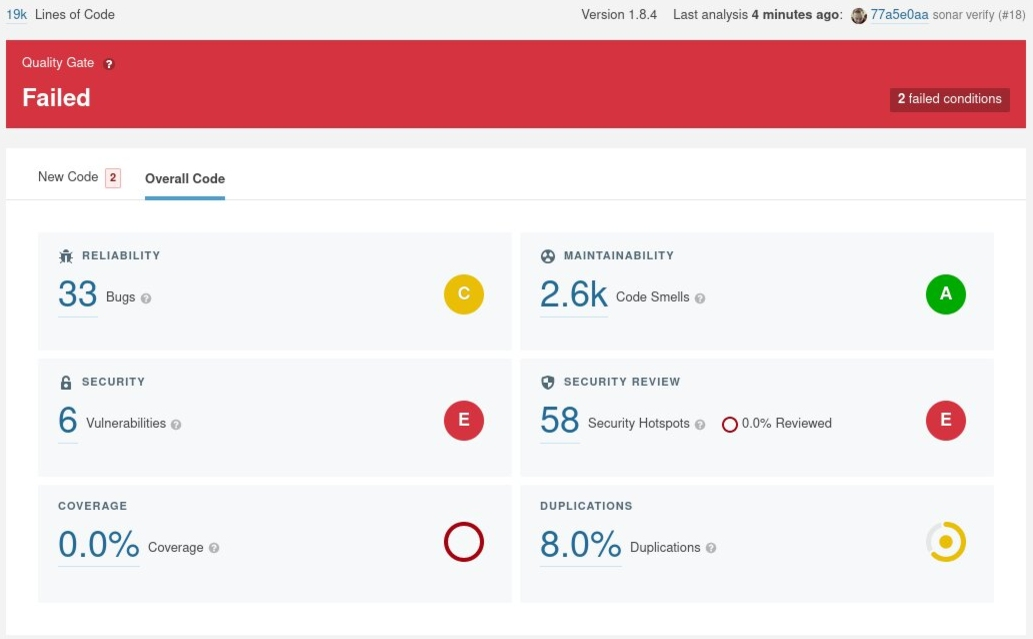
\includegraphics[width=\textwidth]{first_sonar2.jpg}
    \caption{SonarCloud erste Sichtung}
    \label{fig:my_sonar1}
\end{figure}

\begin{figure}
    \centering
    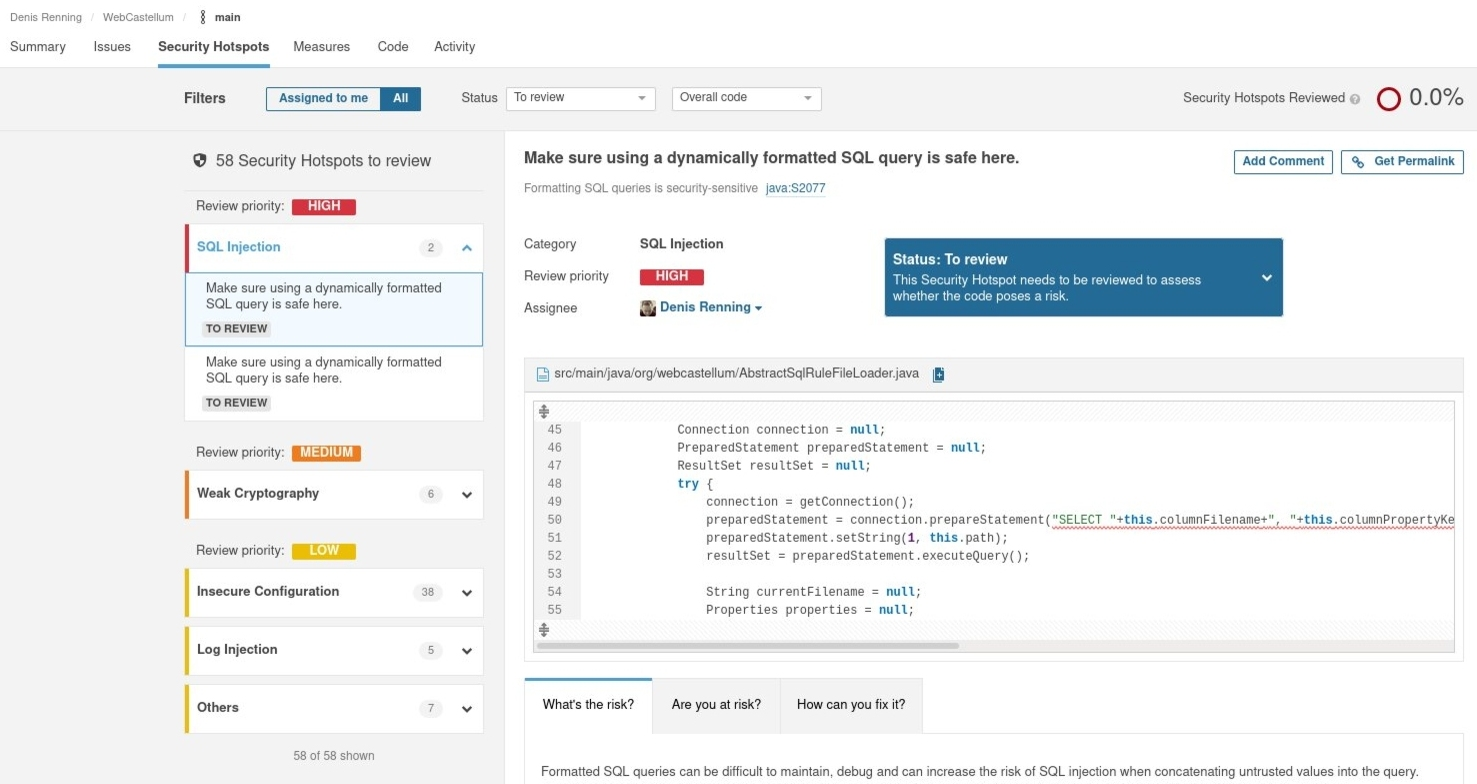
\includegraphics[width=\textwidth]{first_sonar_sql.jpg}
    \caption{SonarCloud SQL-Injection}
    \label{fig:my_sonar2}
\end{figure}



\subsection{ToDos, Unit-Tests,  etc.}

Interessant war ebenfalls die Suche nach \verb=TODO=-Markierungen im Quelltext. Insgesamt 243 mal traten entsprechende Kommentare im Quelltext auf und markierten Stellen an denen die Entwickler Probleme und Verbesserungen vermuteten bzw. Aufgaben für die nächste Version notierten. Diese Notizen reichten von einfachen Aufgabenstellungen, wie \glqq\emph{add proper logging}\grqq, über Refactoring-Ideen bis hin zu Anmerkungen deren Umsetzung die Funktionsweise des Filters beeinflussen würden. \anno{Zitierung aus eigener unveröffentlichter notwendig?}

Einige der Todo-Anmerkungen ließen auf eine geplante Überführung des Quellcodes von Java in der Version 1.4 auf Java 5 schließen. Häufig fanden sich auch auskommentierte dementsprechende Fragmente und, insbesondere bei der Verwendung listenähnlicher Objekte, fallen die in Java 5 eingeführten \emph{Generics} (s. Abbildung \ref{fig:my_l2} auf.

\begin{figure}[h]
  \begin{small}
    \begin{lstlisting}[language=java]
    // TODO: in Utility-Klasse packen (ServerUtils)
    private static void concatenateParameterMaps(
      final Map/*<String,String[]>*/ parameters, 
      final Map/*<String,String[]>*/ parameterMapToAdd) {
    \end{lstlisting}
  \end{small}
  \caption{Auszug aus WebCastellumFilter als Beispiel für ToDos und auskommentierte Generics}
  \label{fig:my_l2}
\end{figure}
  
Dabei sollte berücksichtigt werden, dass diese Kommentare aus dem Jahr 2009 stammen und auch die Programmiersprache Java in den letzten Jahren deutliche Fortschritte gemacht hat. Die Sprache erlaubt mittlerweile auch Konstrukte wie Lambda-Expressions (Java 8) und Typinferenz (Java 10). Ein Refactoring des Quelltextes diesbezüglich wäre sicher lohnenswert.

Tests, im Sinne von Unit-Tests z.B. im Rahmen eines etablierten Testframeworks, lassen sich in den Quellen der Version 1.8.3 nicht finden. Für eine Software, die zur Sicherheit von Anwendungen beitragen sollte, eher ungewöhnlich. Stattdessen existieren in einigen Klassen \verb=main=-Methoden mit entsprechender Absicht. Die Klasse \verb=LargeFormPostRequestTester= dient beispielsweise ausschließlich Testzwecken. \verb=ResponseUtils= behinhaltet gleich fünf auskommentierte \verb=main=-Methoden zum Testen verschiedener Funktionalitäten inklusive der Anmerkung \emph{for local testing only}. 


\subsection{Fehlerbereinigung}

Die minimale (persönliche) Anforderung an das Ziel der Vorarbeiten war den seit 2009 nicht bearbeiteten Quelltext auf eine fehlerfreie Basis anzuheben, ein (kompilierbares) nutzbares Endprodukt zu erhalten und mindestens einen Anwendungsfall eines Angriffs komplett durchtesten zu können.

Umgesetzt wurde dann ein leichtes Refactoring und die Erstellung von 222 Unit-Tests\footnote{\url{https://github.com/devtty/webcastellum/actions/runs/5441412243/jobs/9895332455\#step:8:437} aufgerufen am 07.07.2023}. Dabei wurden:

\begin{itemize}
    \item 33 Bugs beseitigt
    \item 6 Sicherheitslücken beseitigt
    \item 54 Security-Hotspots überprüft
    \item über 300 Code-Smells beseitigt
    \item und die Testabdeckung des Quelltextes von 0 auf 18,8 Prozent angehoben.
\end{itemize}

Zwei Testklassen (\verb=WebFilterDroneTest= und \verb=WebFilterHttpClientTest=) mit insgesamt 14 Tests spielen dabei den Anwendungsfall eines Angriffs per SQL-Injection auf eine kleine Beispiel-Anwendung durch und überprüfen die korrekte Funktionalität des Filters. Mit Hilfe der Arquillian-Erweiterungen \emph{Drone} und \emph{Graphene} wird im Fall der ersten Testklasse ein Browser instantiiert und der Angriff automatisiert über diesen durchgeführt. Im zweiten Fall geschieht dieses, mit Hilfe eines leichtgewichtigen Clients, direkt über das HTTP-Protokoll.

\begin{figure}[h]
    \centering
    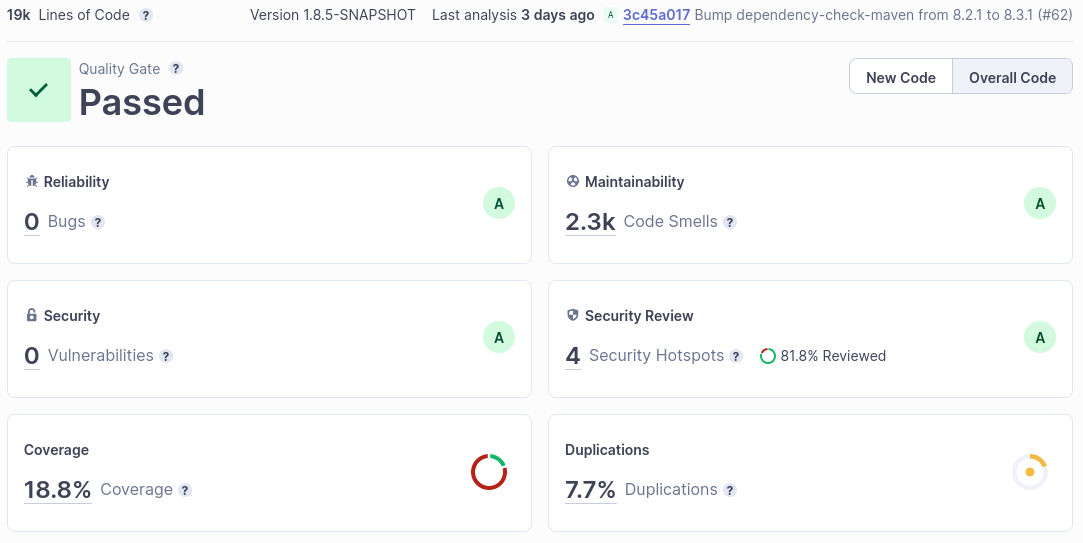
\includegraphics[width=\textwidth]{scfinalc.png}
    \caption{Ergebnis des Bugfixings (Juni 2023)}
    \label{fig:my_sonarf}
\end{figure}

Mit der Möglichkeit der Überwachung der qualitativen Metriken der Anwendung und der erweiterten Testabdeckung können die Arbeiten zur Erweiterung der Web Application Firewall beginnen. Hierzu zählen insbesondere der Datenaustausch zwischen verschiedenen Instanzen über eine zentrale Komponente und die (hoffentlich) effektivere Angriffserkennung.

% Highlight 2 der Implementierung
\section{Zentralisierung}
Im Ursprungszustand handelt es sich bei WebCastellum um einen relativ leichtgewichtigen Servlet-Filter der sämtliche Abwehrmaßnahmen direkt verarbeitet. Abgesehen von den Interaktionen mit der eigentlichen Anwendung existieren nur wenige Berührungspunkte mit externen Systemen. Die zwei wichtigsten Fälle sind dabei die \emph{Konfiguration} der Anwendung und die \emph{Benachrichtung} des Betreibers über den Zustand (Funktion, Angriffe, usw.) der Web Application Firewall. Beide Fälle benutzen derzeit textuelle Schnittstellen. Die Konfiguration erfolgt über \emph{manuelles} Editieren des Bereitstellungsdeskriptors (\emph{web.xml}) und die Bereitstellung des Status über Logdateien. Um den Datenaustausch mehrerer Instanzen der WAF nach dem Muster aus Abschnitt~\ref{sec:zentralisierungkern} zu ermöglichen, müssten zusätzliche (maschinell lesbare) Schnittstellen geschaffen werden. Diese Schnittstellen sorgen dann für den Datenaustausch mit einer zentralen Schnittstelle (Abbildung~\ref{fig:my_verbund}).

\begin{figure}[h]
    \centering
    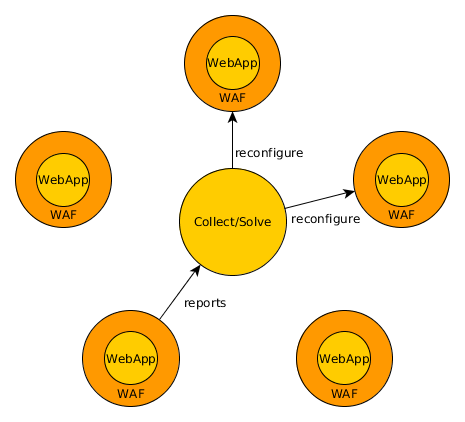
\includegraphics[width=8cm]{central.png}
    \caption{Arbeit der WAFs im Verbund}
    \label{fig:my_verbund}
\end{figure}

Glücklicherweise haben die Entwickler der WebCastellum-Software entsprechende Schnittstellen (nun im Sinne der objektorientierten Programmierung) mitgeliefert. Das System bietet mit dem Interface \verb=org.webcastellum.ConfigurationLoader= sozusagen bereits eine technische Blaupause für die Implementierung einer alternativen Konfigurationsmöglichkeit. Tatsächlich finden sich in der Software bereits zwei Implementierungen des \emph{Interfaces}:

\begin{description}
  \small
\item[DefaultConfigurationLoader] \hfill \\
  lädt die Konfiguration, wie zuvor beschrieben, aus Parametern im Bereitstellungsdeskriptor (\emph{web.xml})
\item[PropertiesFileConfigurationLoader] \hfill \\
  lädt die Konfiguration aus einer benannten Datei im \emph{properties}-Format mit der Möglichkeit bei fehlenden Werten auf die Daten der \emph{web.xml} zurückzufallen.
\end{description}

Zusätzliche Implementationen der Schnittstelle könnten sich die Konfigurationsparameter über beliebige Quellen, zum Beispiel in Form eines REST-API-Clients, \glqq\emph{besorgen}\grqq. 


\begin{figure}[h]
  \begin{center}
    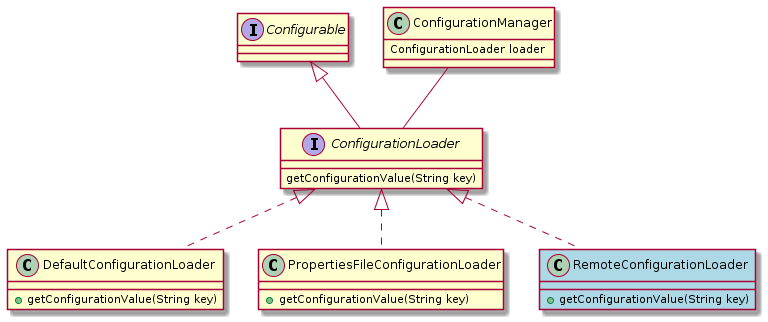
\includegraphics[width=14cm]{configclasses}
    \caption{Implementierung Konfiguration}
    \label{fig.impkonfig}
  \end{center}
\end{figure}



\begin{figure}[h]
  \begin{center}
    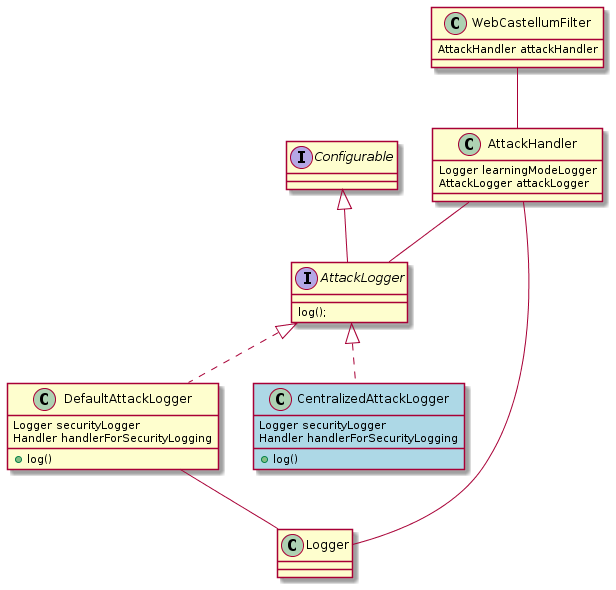
\includegraphics[width=12cm]{classp}
    \caption{Implementierung Nachrichtenversand}
    \label{fig.impversand}
  \end{center}
\end{figure}




\section{ML-Fähigkeit}

Die Implementierung der ML-Fähigkeit erfolgt nach dem Vorschlag aus \cite{kozik2014}.

Aus den Testdaten werden dafür nur die Attribute der URL, der HTTP-Methode und die Payload (die Requestparameter) genutzt. 

Klassifizierung anhand der J48-Implementierung eines Entscheidungsbaums nach dem C4.5-Algorithmus

\begin{figure}[h]
    \centering
    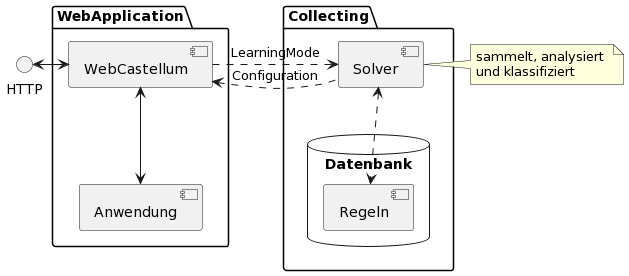
\includegraphics[width=9cm]{webcastellumcentral.png}
    \caption{Komponentendiagramm für zentrale Klassifizierung}
    \label{fig:my_future}
\end{figure}

\section{Lernmodus}

% Highlight des Deployments beim Kunden

% Zusammenfassung: ca. 0,5 Seiten
\section{Zusammenfassung}

% Was haben wir in diesem Kapitel gelernt?
% Wie passt das zur Zielstellung der Arbeit?
% Wie passt das zum nächsten Kapitel?